\documentclass[10pt,twocolumn]{article}
\usepackage{amsthm, amssymb, geometry, mathrsfs}
\usepackage[T1]{fontenc}
\usepackage{graphicx}
\usepackage[utf8]{inputenc}
\usepackage[style=ieee]{biblatex}
\addbibresource{citations.bib}
\usepackage{multicol}% http://ctan.org/pkg/multicols

\title {Multi-Class Classification of Scientific Articles}
\author {Xavier Denis, Andrew Doyle, Kashif Javed}

\begin{document}
\maketitle
\section*{Abstract}

Classification of text documents has been well-studied for some types of text, but state-of-the-art algorithms have not been tested on scientific journal articles.  A study was performed on a new, large dataset consisting of abstract text for four types of articles: computer science, statistics, physics and math. A baseline Naive Bayesian classifier is compared to the more advanced k-Nearest Neighbours and Random Forest classifiers, with an emphasis on feature extraction and selection techniques.

\section*{Introduction}

Categorization of articles in scientific journals is a useful step towards making it easy for future researchers to find and build upon the body of knowledge in their field. Normally, it is fairly obvious to a human editor how to categorize a new article, so an automated system to classify documents is unnecessary.  However, with the rise of open access journals, more and more articles are being indexed into journals other than the ones they were published in, which might use a different categorization scheme.  When a one-to-one mapping of categories is impossible, it can be time-consuming to review large numbers of articles and find a suitable category from within the new categorization.

\section*{Related Work}

The problem of automatic text classification using machine learning has been extensively studied on several datasets, including the 20 Newsgroups dataset and the Reuters dataset.  The 20 Newsgroups dataset included a collection of almost 20,000 newsgroup threads from twenty different categories.  Some of the categories are closely related, such as ``rec.sport.baseball'' and ``rec.sport.hockey'', and some categories have nothing to do with the others, such as ``misc.forsale''.

The Reuters-21578 dataset provides a similar number of news articles with corresponding categories for machine learning research.  Released in 1990, it provides a different type of text, given that the 20 Newsgroups are dicussions from internet users and the Reuters articles are news broadcasts not meant for interaction.  The Reuters-21578 dataset has been superceded by the RCV1 dataset, which contains over 800,000 labeled news articles.

The dataset under consideration here is different in that the full text of the articles are not available; only a part of the complete data is available, the abstract.  The prediction task is to classify each abstract as a computer science, physics, statistics, or math paper.

\section*{Data Pre-processing}

Simple transformations were performed on the raw data to normalize it and extract the most meaning. A further stage of transformations was performed at the corpus level on the ensemble of extracted features.

\subsection*{Latex Removal}

Mathematical equations in latex generally appear as a mathematical expression between two \$ symbols. The primary issue with this latex formatting is that semantically similar phrases can take very different and hard to parse appearances. To remove this kind of formatting, all text between two matched \$ symbols was extracted. All instances of mathematical expressions are replaced by a symbol: $math123$. In this way, mathematical expressions are simply counted, and this count used as a feature, rather than each component of the expression parsed and used as individual features.  This produces features that are more easily comparable across documents and categories.

\subsection*{Text Normalization}

After removing all latex formatting, the text is normalized using standard techniques[cite]. First the entire document is transformed to lowercase, reducing vocabulary size significantly. Next, it is broken up into word chunks by spaces, removing all punctuation in the process. Theses two approaches can reduce the size of the vocabulary significantly. A Porter stemmer [cite] was employed to reduce words to their root.  For example, after stemming, the words ``quantum'' and ``quanta'' are considered equivalent, and counted together. The Porter stemmer groups different verb tenses, adjectives and nouns that have identical semantic meaning, and plurals of words.  The main advantage of employing the Porter stemmer is the reduction of sparsity of the features by grouping features into semantic groups.  It was found that using the stemmer reduced the size of the corpus vocabulary by approximately $25\%$.  To further reduce the size of the vocabulary, words of length less than 4 characters were discarded, which reduced our feature space by approximately $20\%$.  As the final step to pre-processing the abstract data, a list of English stop words, was filtered out of our feature matrices.  These stop words represent the most common words in the English language, and are assumed not to have any information about the contents of the document.  For example, words like ``a'', ``then'', and ``but'' cannot be expected to contain information about what type of document they appear in, but may appear to correlate to one of the classes in the training set and result in overfitting.  Figure 1 shows the 20 most frequent words in the dataset longer than 3 characters, including stop words, and with the possible exception of ``algorithm'', none of them are very indicative of a categorical context.

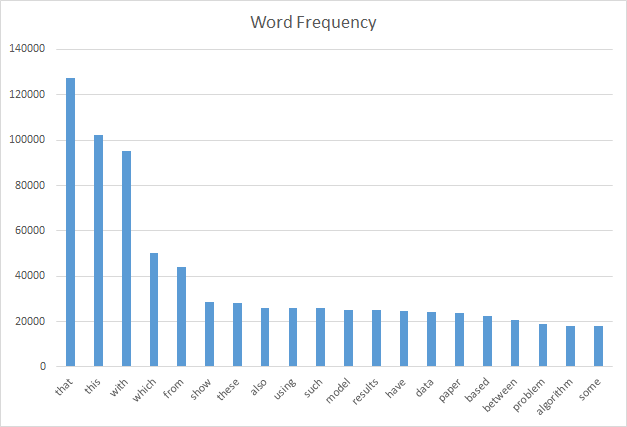
\includegraphics[width=0.5\textwidth]{./word_frequency.png}

\section*{Feature Design and Selection}

After raw data was pre-processed using the above steps, two sets of features were considered: word count, and TF-IDF.

\subsection*{Word Count}

\begin{figure}
  \centering
  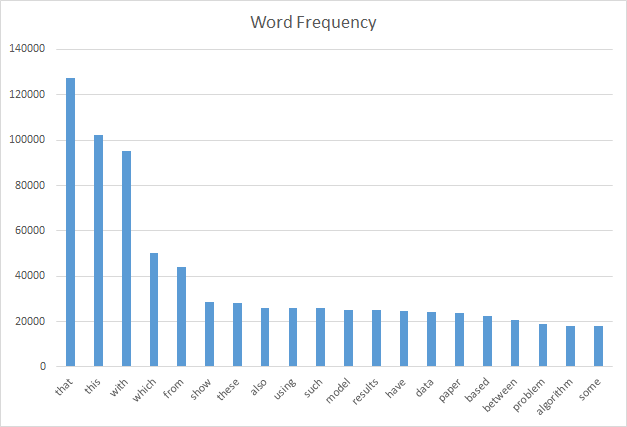
\includegraphics[width=0.5\textwidth]{./word_frequency.png}
  \label{freq}
\end{figure}

This type of feature is simple, consisting of the word counts $n_{wd}$ in each document for all words. From this set of features, the instances of words across an entire class can easily be computed, and used in Naive Bayes classification to estimate $P(w | c)$ for every word $w$ and class $c$. The set of all words, even after stemming and filtering, was too large to be used in the scikit-learn classifiers, so several strategies were employed to select the best word counts.  First, the 2000 most frequently appearing words were selected, and found to give fairly good performance with the scikit-learn random forest classifier.  A qualitative assessment of these words assessed that many of the most common words contained no semantic information, and that the optimal feature set might lie with less frequent words that appeared in only one of the classes, so an arbitrary number of most frequent features was skipped, and the next 2000 features used.  This was found to decrease the quality of prediction, but an exhaustive search of the feature space was not performed due to the promise of TF-IDF features.

\subsection*{TF-IDF}

Term Frequency-Inverse Document Frequency calculates $n'_{wd} = \log (n_{wd} + 1) \times log (|D| / df(w))$ where $df(\cdot)$ is the \emph{document frequency} of a word, or the number of documents containing a word. The purpose of this transformation is to compensate for the influence of common words and emphasize the influence of rare ones in word counts. While TF-IDF can compensate for rare and frequent words it does not consider document length. Document length is normalized by dividing the feature vector by the average document length, according to the $L_2$ Norm.

A second transformation that was explored is a class-length prior distribution for word frequencies. Word frequencies for each class were scaled by the total word count within the class. The purpose of this rescaling is to consider the words in a manner purely relative to their own class, rather than in comparison to other classes.

When classifying text with kNN, the dimensionality of the vector space is problematic. Although the distance metric employed accomodates higher dimensions more easily, when faced with the dimensions of the word space, some form of feature selection is required.

\subsection*{SVD}

Singular value decomposition is a technique that will break a matrix $M$ into three matrices $U, S, V^T$ such that $U \cdot S \cdot V^T = M$. The use of SVD in feature selection is that reducing the rank of the diagonal matrix $S$ to $k$, it will produce the closest matrix $M'$ of degree $k$ to $M$. By interpreting the feature vectors as a document-feature matrix, or in this case as a tf-idf matrix, we can find the best features. 

The main obstacle encountered using SVD is that allowable python packages for this project do not have efficient implementations. Calculating the SVD for a matrix of 96,000 rows by approximately 88,000 columns took approximately 1 hour and required several gigabytes of RAM to store the three output matrices. Additionally, since the kNN classification suffered from slow performance, adding matrix multiplication to each distance calculation would further reduce throughput.

Additionally, there is no theoretical evidence that using the features with highest values in the $S$ matrix will be the best features in classification.

\subsection*{Random}

In research done for this work, a conclusive strategy for selecting a subset of features was not determined, so selecting a random subset was attempted as a baseline.  Selecting the optimal $k$ features could be accomplished using cross-validation or gradient descent, but not implemented in this work.

\subsection*{Most Frequent}

Another strategy for selecting the optimal set of features could be to pick the $k$ most frequent words. This approach has several obvious problems. First, and most obvious is the issue of stop words, words which are frequent but carry little meaning. While TF-IDF will give a low score to these words, choosing the $k$ most frequent words will ignore these scores. Second, this method of selection assumes that the most frequent words contain the most information about document class. It ignores situations where two seperate terms may by highly correlated with half of each class but not in the $k$ most frequent words. These problems can be mitigated by filtering out stop words ahead of time and experimenting with values of $k$ but will never completely disappear.

\section*{Algorithm Selection}

The types of algorithm usable for text classification are limited by the large feature space. Several types of algorithms have shown good performance in the literature, including: LLSF, Multinomial Naive Bayes, Decision Trees, and kNN. A multinomial Naive Bayesian classifier was implemented to measure baseline performance for the different feature selection strategies. Naive Bayes is known for high performance in text envirnoments since its structure allows for efficient learning of large numbers of features.

\subsection*{Baseline: Naive Bayes using word counts}

In order to establish a baseline for future algorithms, the simplest version of Naive Bayes was implemented. Naive Bayes estimates the probability $P(c|w)$ through the use of Bayes Rule.

\[ \frac {P(c)P(w|c)} {P(w)} \]

While $P(c)$ can be estimated easily by counting the raw occurences of the label $c$ within the training data, $P(w|c)$ requires more work. $P(w|c)$ is estimated by the following formula:

\[\frac {\sum_{d \in D_c} n_{wd}} {\sum_{w'} \sum_{d\in D_c} n_{wd}} \]

While performing sums is efficient for a computer, calculating the denominator on the entire training set can prohibitive with $O(mn)$ for $m$ features and $n$ documents. To solve this issue, the sums are reversed, taking advantage of the sparsity of features within documents. While the same order-bound is preserved, given that a single abstract will not contain more than a few hundred unique words, less iterations are expected.

\subsection*{Standard: Naive Bayes with TF-IDF and kNN with TF-IDF}

For the `standard' approach, the use of TF-IDF features was explored with multinomial naive bayes and k-Nearest Neighbours classifiers. Another approach considered was Text Weighted Complement Naive Bayes.

For Naive Bayes, rewriting the algorithm to operate on a two dimensional document-feature matrix rather than the actual class based word counts allows changing the features. By doing so, raw word counts can be replaced with TF-IDF values. 

kNN attempts to search for the $k$ nearest points to the query point. The first step then, is to define some metric (distance) function. For this, the cosine similarity of TF-IDF vectors was used,

\[
sim(A,B) = \frac {\sum_{w \in A \cap B} A_w \times B_w} {\| A \| \| B \|}
\]
Where $A,B$ are TF-IDF vectors. Once the metric function is defined, kNN simply becomes a matter of iterating over the training set to find the $k$ documents with the highest scores. To label a test document, the most frequent of the $k$ nearest labels is chosen.

The primary difficulty with kNN is that each query will be computationally expensive, because each test sample must be compared to every sample in the training set. Due to this requirement, the trick used for efficiency in Naive Bayes couldn't be used, requiring an inner loop of 80,000 iterations if all the training data is used. This issue is why feature selection and reduction is paramount in kNN, since it will significantly reduce computation time.

\subsection*{Advanced: Random Forests}

Random forests have produced excellent results in many classification contexts. The scikit-learn random forest classifier, using the 1,500 most frequent word counts as features, classified the test set with $82\%$ accuracy. To obtain this result, only 50,000 of the ~70,000 available training examples were used because of memory limitations, with 150 estimator trees.  Increasing the number of training samples used, the number of features, and the number of trees should improve accuracy, but this was the best result obtainable with the resources available.  An earlier trial, using 10,000 training samples, 100 trees and 1000 features scored $78\%$.

Random forests were not applied to the TF-IDF feature type because of an incompatibility in they way data was stored.

\section*{Parameter Selection}

The classifiers used in this study have few parameters to select, and the most important factor that affected classification was the type of features selected. Increasing the number of features used with Naive Bayes and the Random Forest classifiers improved performance, but were not maximized due to time and technical considerations.

For the kNN classifier, the number of closest training samples, $k$, could be tuned through cross-validation, but due to the time required to classify even one document, a full k-fold validation of this parameter was not performed.

\subsection*{Future Work}

Changing the implementation of the Random Forest word frequency feature to use sparse matrices could allow use of all training data and increase the number of features considered.  

\subsection*{Normalization Length}

Given enough time and resources however, here are some of the most interesting parameters that could be tested.

\subsection*{Feature Vector Length}

The length of each feature vector can be normalized to a specific length. Doing so allows to consider each feature relative to the document it was a part of, rather than the absolute corpus. A side effect is correction for documents of varying lengths since each vector will add up to the same value under the norm used.

\subsection*{Vocabulary size}

Algorithms such as kNN suffer heavily from dimensionality, with performance dropping dramatically as the number of dimensions grows. In text classification, the number of features can easily reach over a hundred thousand, and kNN would be rendered useless. Trimming the size of the word dictionary used can force specific words to be emphasized.

\subsection{Testing and Validation}

\subsection*{k-fold X-Val}

\begin{figure}
  \centering
  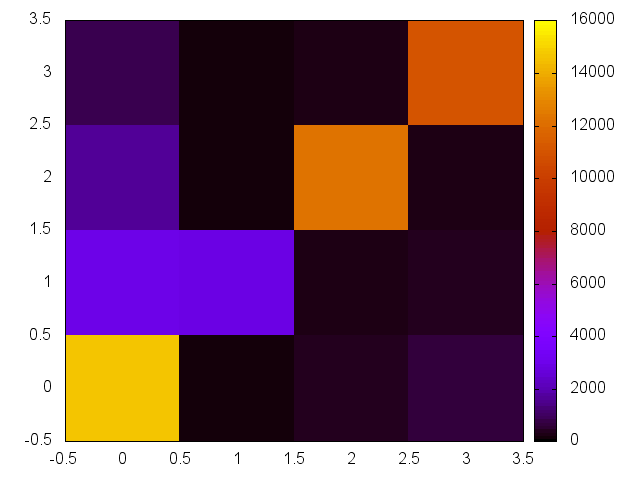
\includegraphics[width=0.5\textwidth]{./confusion.png}
  \label{confusion}
\end{figure}
\begin{figure}
  \centering
  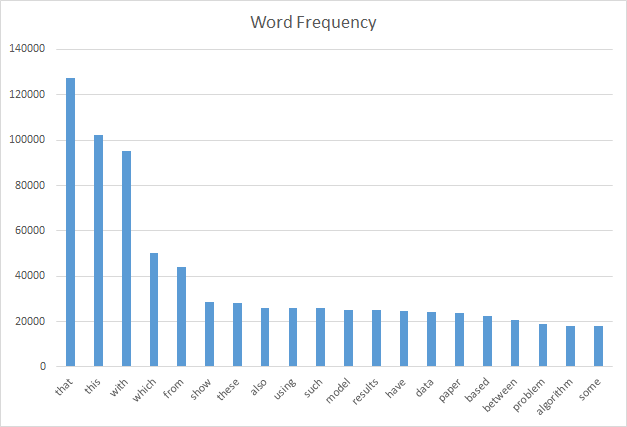
\includegraphics[width=0.5\textwidth]{./word_frequency.png}
  \label{freq}
\end{figure}
\begin{figure}
  \centering
  \begin{tabular}{|l || r|}
  \hline
  Feature & Mis-Classifcation\\
  \hline
  Word Count     & 0.133135848664 \\
  TF-IDF         & 0.146835048332 \\
  TF-IDF$_a$     & 0.149942833385 \\
  Word Count$_a$ & 0.145837231057 \\
  \hline
  \end{tabular}
  \caption {Mis-Classification rates for different features used by Naive Bayes. The $a$ subscript indicates that the feature vectors were length normalized. All values were calculated after 10-fold cross-validation on the entire training set.}
\end{figure}


\section*{Discussion}

Overall, classification was relatively accurate with an $87\%$ TP rate acheived on the public Kaggle data. However, a few mistakes were made that could have impacted performance of the algorithms. Using the vocabulary of the test data can help extract features that will only be relevant to that data.  While in a more general setting this could easily lead to overfitting and pollution of error estimates, since all the test data was available, overfitting could lead to better results. 

\subsection*{Statistics Confusion}

Additionally, as the ROC curve shows, there is an issue classifying the statistics papers. Investigating the source of this issue could have led to reducing error rates dramatically. Two possible sources of confusion could be undersampling in Statistics and high correlation between Statistics and CS vocabularies.

\subsection*{kNN performance}

While kNN is known for slow querying speed, the actual speed was not expected to be so low. This low throughput limited the exploration of kNN since the Python implementation took an estimated 23 hours to generate a Kaggle submission. For this reason, many of the interesting optimizations and choices with kNN were glossed over. Literature reviews suggest that given resources and time to run the actual algorithm performance can be quite high[cite].

\subsection*{Difficulty of TF-IDF}

While TF-IDF can seem like a silver bullet when dealing with unfiltered word counts, it can actual bring it's own issues. The first is that it can add a decent amount of additional work if document frequencies are calculated as their own step. Computation times can be annoying but are easily dealt with through more advanced hardware. The most important issue however, is that if words are not tokenized properly and many unique words are introduced, then scores can become problematic. Additionally, by forcing Naive Bayes to use a possibly transformed \emph{document-feature} matrix, more work is required to count the class frequencies required.


\end {document}
